%%%%%%%%%%%%%%%%%%%%%%%%%%%%%%%%%%%%%%%%%%%%%%%%%%%%%%%%%%%%%%%%%%%%
%% I, the copyright holder of this work, release this work into the
%% public domain. This applies worldwide. In some countries this may
%% not be legally possible; if so: I grant anyone the right to use
%% this work for any purpose, without any conditions, unless such
%% conditions are required by law.
%%%%%%%%%%%%%%%%%%%%%%%%%%%%%%%%%%%%%%%%%%%%%%%%%%%%%%%%%%%%%%%%%%%%

\documentclass{beamer}
\usetheme[faculty=fi]{fibeamer}
\usepackage[utf8]{inputenc}
\usepackage[
  main=english, %% By using `czech` or `slovak` as the main locale
                %% instead of `english`, you can typeset the
                %% presentation in either Czech or Slovak,
                %% respectively.
  czech, slovak %% The additional keys allow foreign texts to be
]{babel}        %% typeset as follows:
%%
%%   \begin{otherlanguage}{czech}   ... \end{otherlanguage}
%%   \begin{otherlanguage}{slovak}  ... \end{otherlanguage}
%%
%% These macros specify information about the presentation
\title{Introduction to Manifold Learning} %% that will be typeset on the
\subtitle{A Geometry View on Machine Learning} %% title page.
\author{Xiaoyu Xue}
%% These additional packages are used within the document:
\usepackage{ragged2e}  % `\justifying` text
\usepackage{booktabs}  % Tables
\usepackage{tabularx}
\usepackage{tikz}      % Diagrams
\usetikzlibrary{calc, shapes, backgrounds}
\usepackage{amsmath, amssymb}
\usepackage{url}       % `\url`s
\usepackage{listings}  % Code listings
\newcommand{\bol}[1]{\textbf{#1}}
\frenchspacing
\begin{document}
  \frame{\maketitle}

  \AtBeginSection[]{% Print an outline at the beginning of sections
    \begin{frame}<beamer>
      %\frametitle{Outline for Section \thesection}
      %\tableofcontents[currentsection]
      \frametitle{Manifold Learning}
      \tableofcontents
    \end{frame}}

  \begin{darkframes}
    \section{Manifold}
    
    \begin{frame}{Manifold Learning}
    \begin{itemize}
    	\item The data space may not be a Euclidean space, but a nonlinear manifold
    	\item Unfold a manifold, and preserve the geometry structure.
    	\item Euclidean distance $\Longrightarrow$ geodesic distance
    \end{itemize}
	\begin{figure}
	\centering
	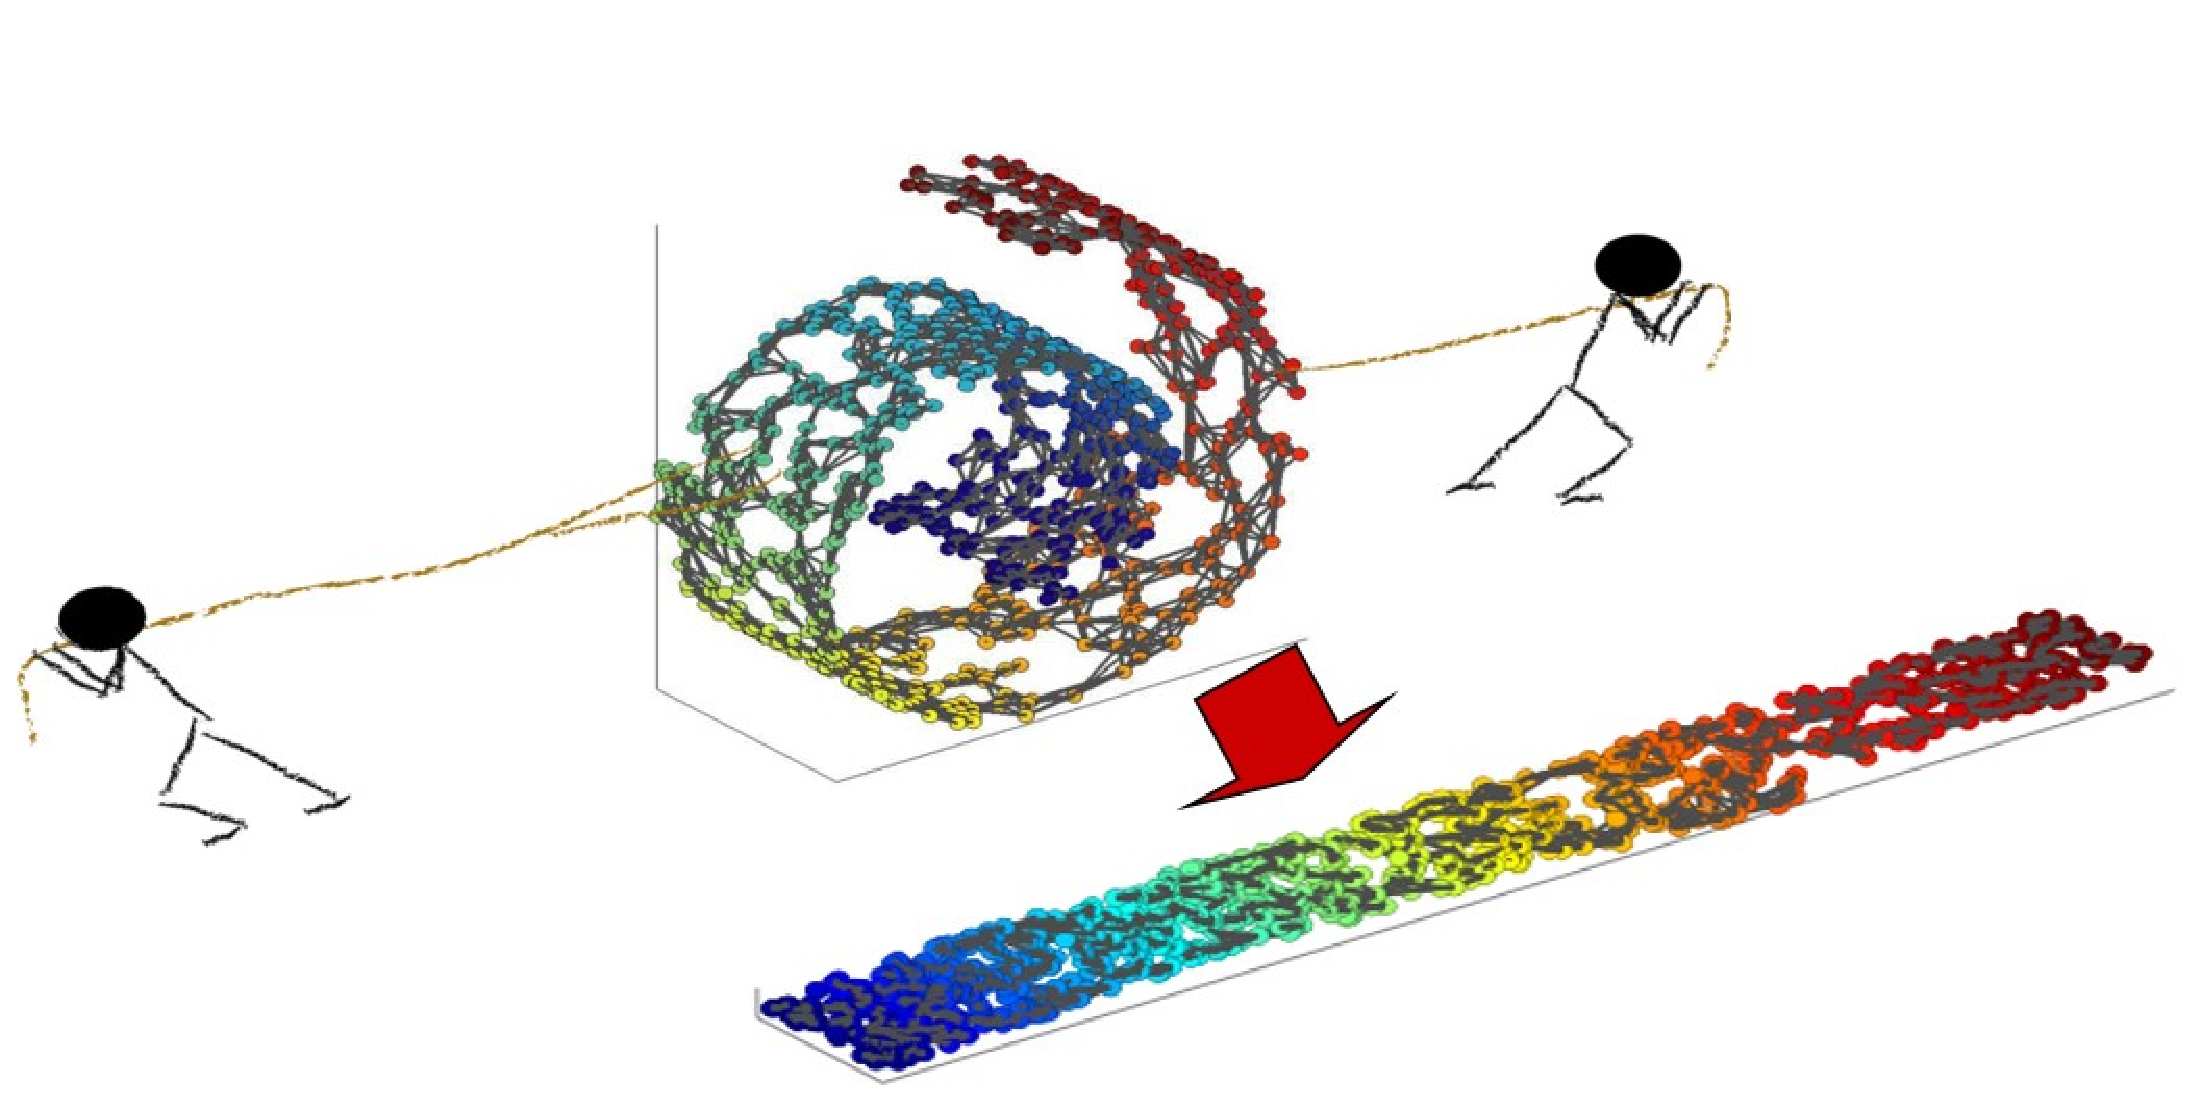
\includegraphics[scale=0.2]{./figs/fig1.eps}
	\end{figure}
    \end{frame}

    \begin{frame}{Manifold Learning}
    Find a Euclidean embedding, and then perform traditional learning algorithms in the Euclidean space.
	\begin{block}{Definition of Manifold Learning}
	Given data points $\bol{x}_1, \ldots, \bol{x}_m \in \mathcal{M} \subset \mathbb{R}^n$, try to find a map $f : \mathcal{M} \to \mathbb{R}^d, d\ll n$, where $f = (f_1, \ldots, f_d), f_i : \mathcal{M} \to \mathbb{R}$
	\end{block}
 	\begin{itemize}
 		\item The manifold is unknown! We have only samples!
		\item How to compute the distance on $\mathcal{M}$?
		\item How to find the mapping function $f$
 	\end{itemize}
    \end{frame}

	\begin{frame}{Manifold of Face Images}
	\begin{figure}
	\centering
	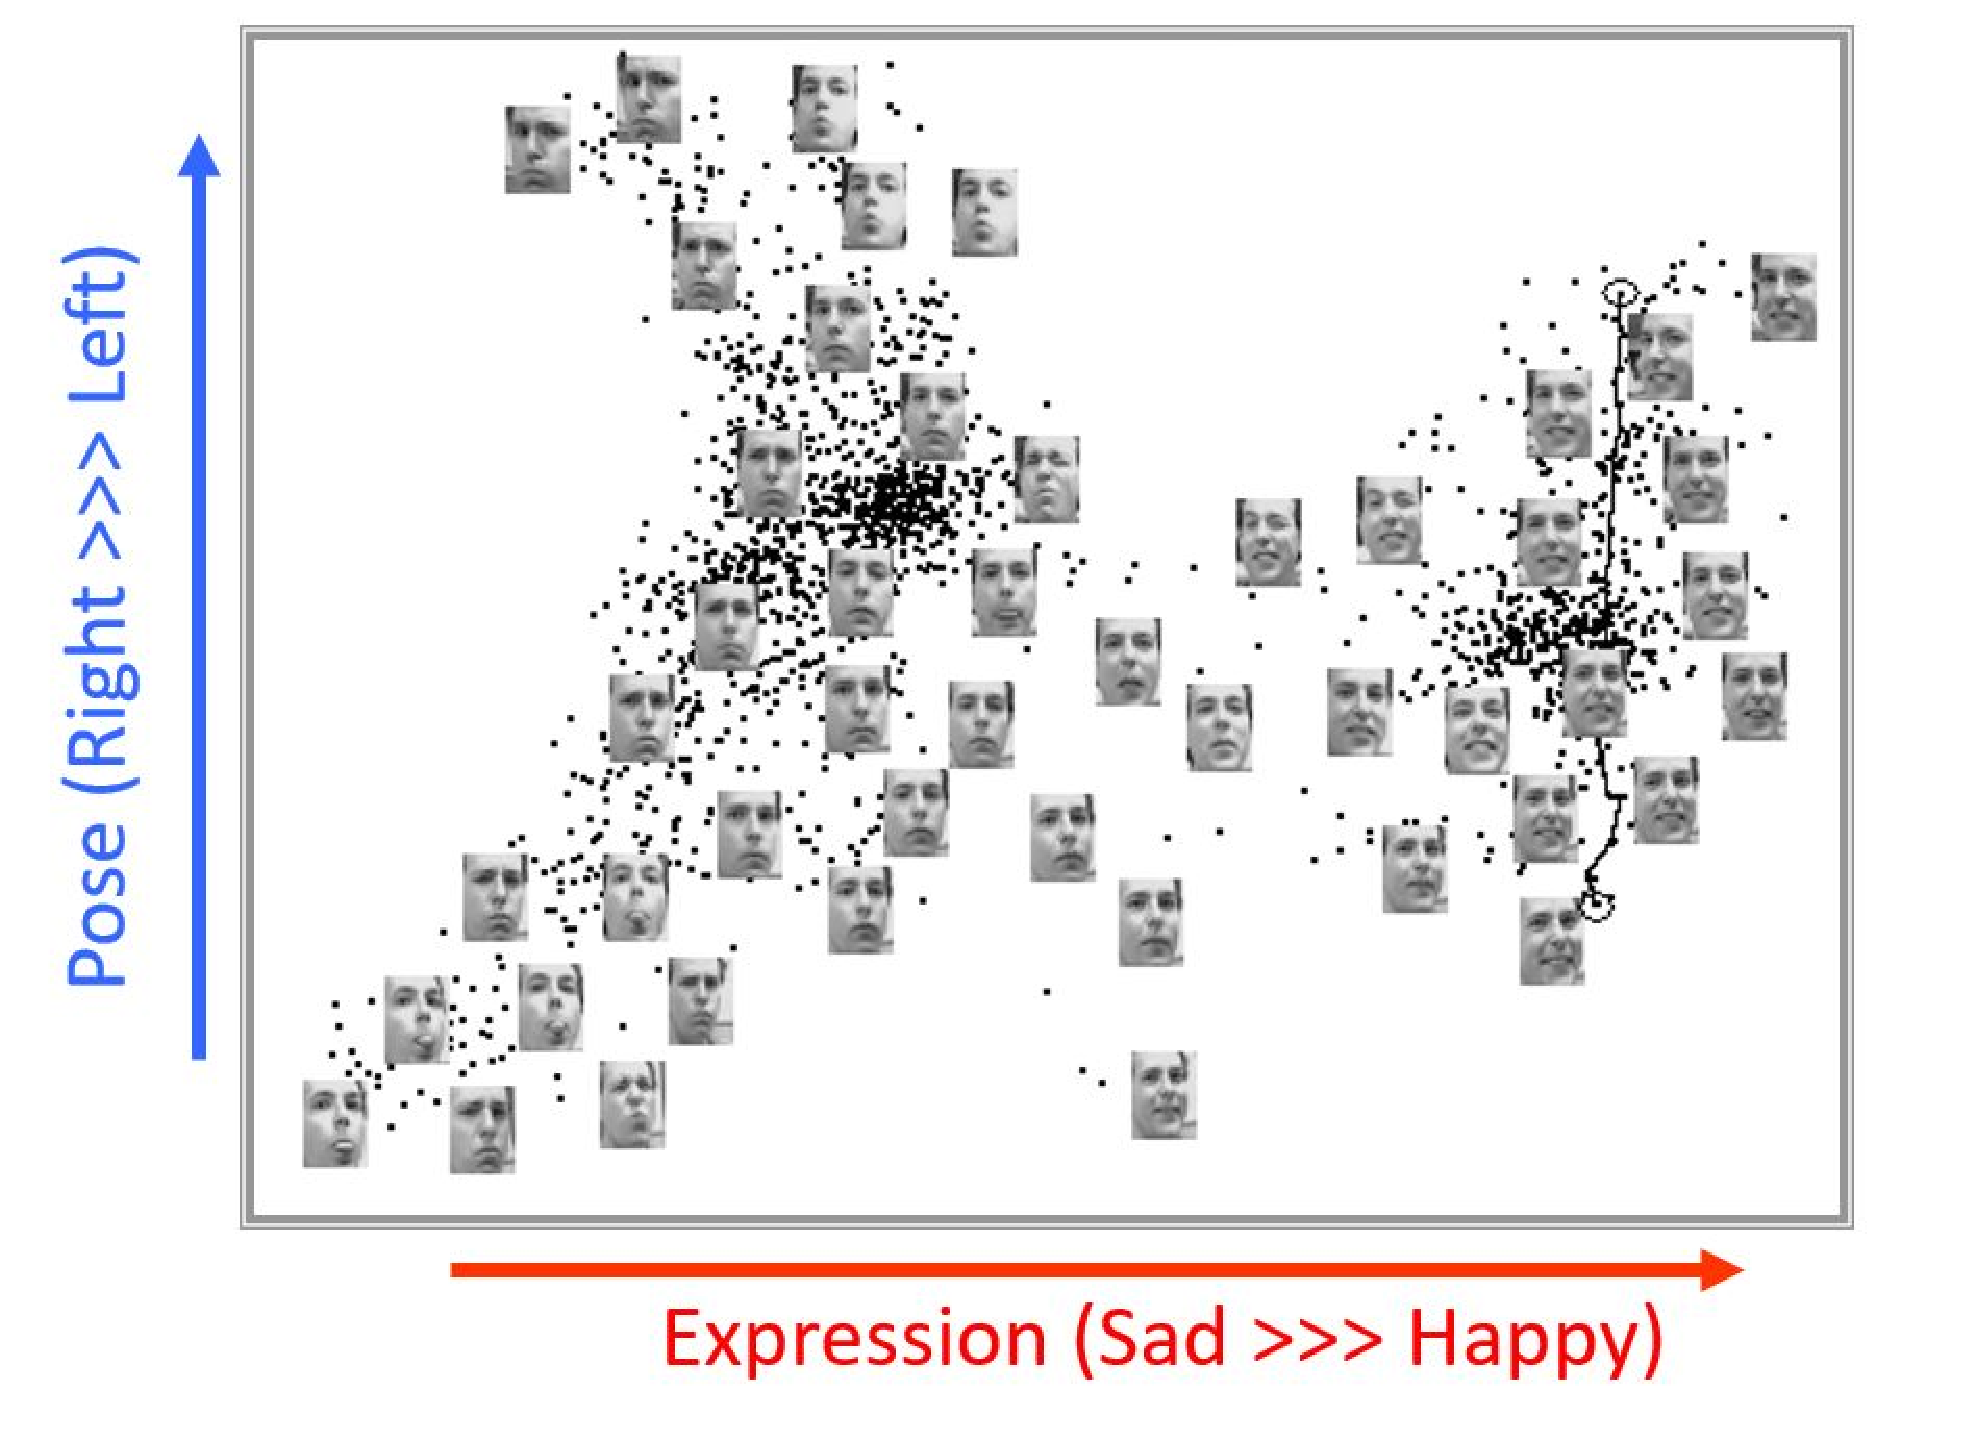
\includegraphics[scale=0.28]{./figs/fig4.eps}
	\end{figure}
	
	\end{frame}
	
	\begin{frame}{Manifold of Handwritten Digits}
	\begin{figure}
	\centering
	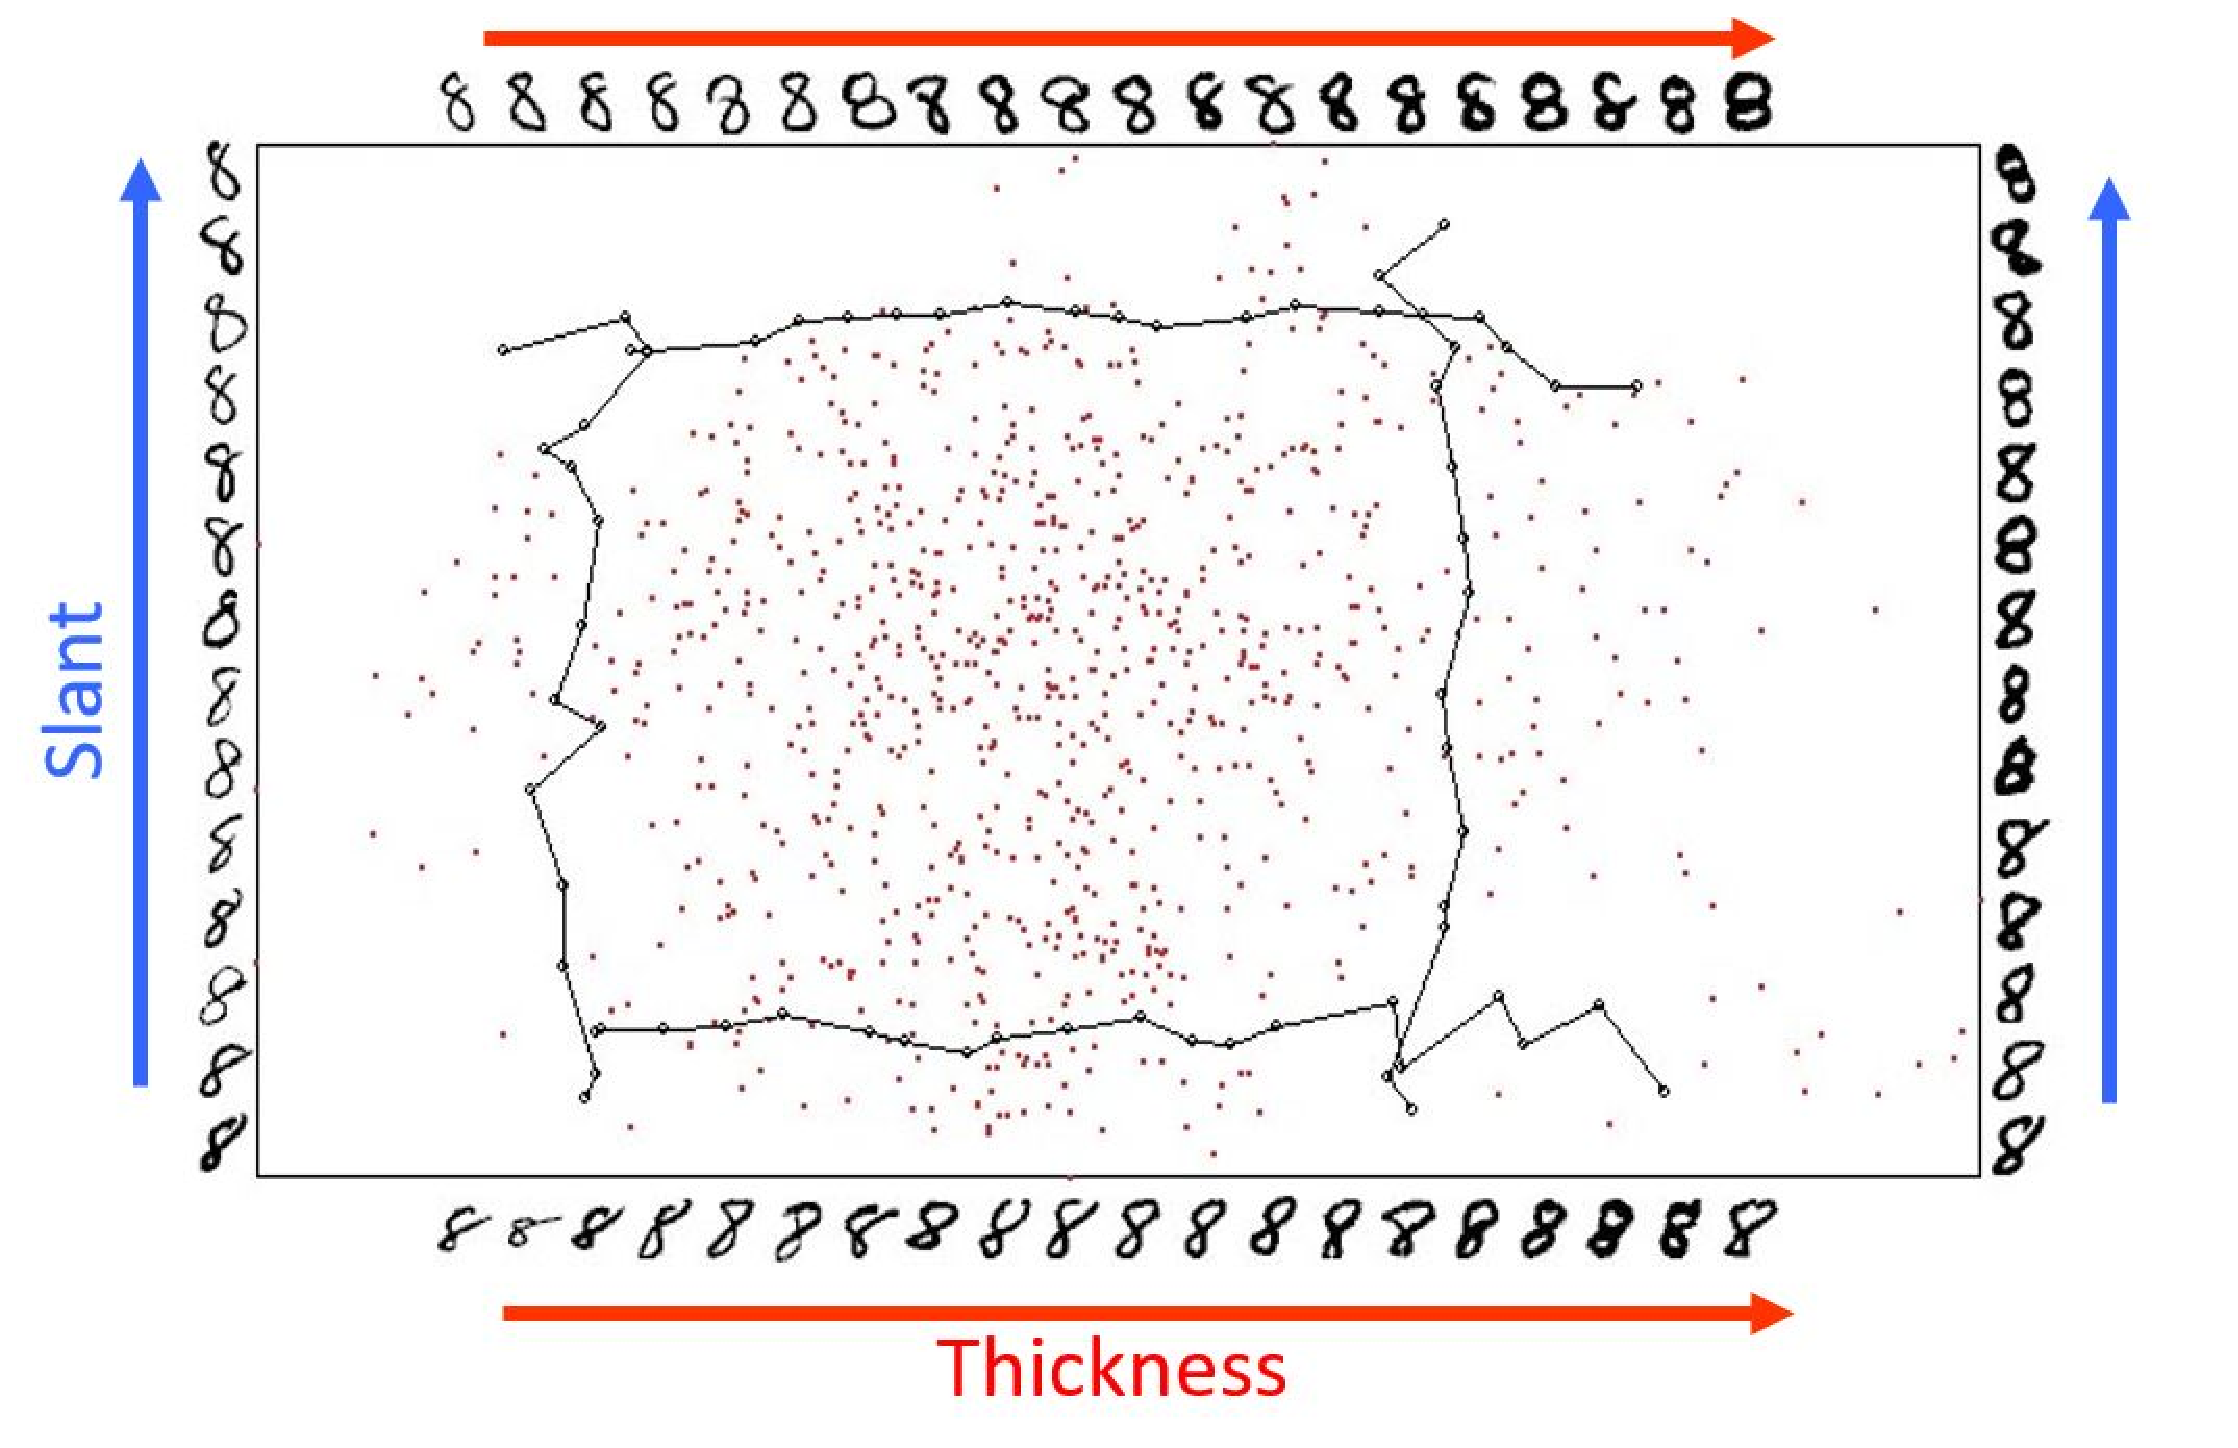
\includegraphics[scale=0.26]{./figs/fig5.eps}
	\end{figure}
	
	\end{frame}	
	
    \section{Manifold based Dimensionality Reduction}
    \subsection{Principal Component Analysis}
    \begin{frame}{PCA: Traditional Dimensionality Reduction Method}
    Principal Component Analysis using linear projection to project data to some directions which have maximum variances
  	\begin{eqnarray*}
  		\bol{p}_{opt} & = & \arg\max_{\bol{p}}\sum_{i = 1}^m(y_i - \bar{y})^2\\
  							& = & \arg\max_{\bol{p}}\bol{p}^TC\bol{p}\\
  							&    &  s.t. \bol{p}^T\bol{p} = 1
  	\end{eqnarray*}
  	\begin{itemize}
  		\item If the manifold is linear, PCA can find the optimal result
  		\item PCA can not process nonlinear manifold
  	\end{itemize}
    \end{frame}
    
    \subsection{Multidimensional scaling}
    \begin{frame}{MDS and ISOMAP}
    \alert{Multidimensional scaling} tries to preserve the Euclidean distances
    \begin{displaymath}
	\Delta :=
	\left( \begin{array}{cccc}
	\delta_{1,1} & \delta_{1,2} & \ldots & \delta_{1,m} \\
	\delta_{2,1} & \delta_{2,2} & \ldots & \delta_{2,m}\\
	\vdots & \vdots & &\vdots\\
	\delta_{m,1} & \delta_{m,2} &\ldots & \delta{m,m}\\
	\end{array} \right)
   \end{displaymath}
   The $\delta$ is the Euclidean distance of every two points $ \delta_{ij}=\Vert \textbf{x}_i - \textbf{x}_j \Vert$ 
   \[
     \min_{\textbf{y}_1,\ldots,\textbf{y}_m} \sum_{i<j}\left(\Vert \textbf{y}_i - \textbf{y}_j \Vert - 
     \delta_{i,j}\right)^2,\quad \textrm{dim}(\textbf{y}_i) \ll \textrm{dim}(\textbf{x}_i)
   \]
    \end{frame}
   
   
   \subsection{ISOMAP}
    \begin{frame}{MDS and ISOMAP}
     \alert{ISOMAP} tries to keep the geodesic distances instead of the Euclidean distances.
    \begin{itemize}
    	\item How to evaluate the geodesic distances with limited samples?
    	\item Construct the adjacency Graph, and calculate the shortest distances (Dijstra or Floyd algorithm)
    \end{itemize}
   	
   	\begin{figure}
   	\centering
   	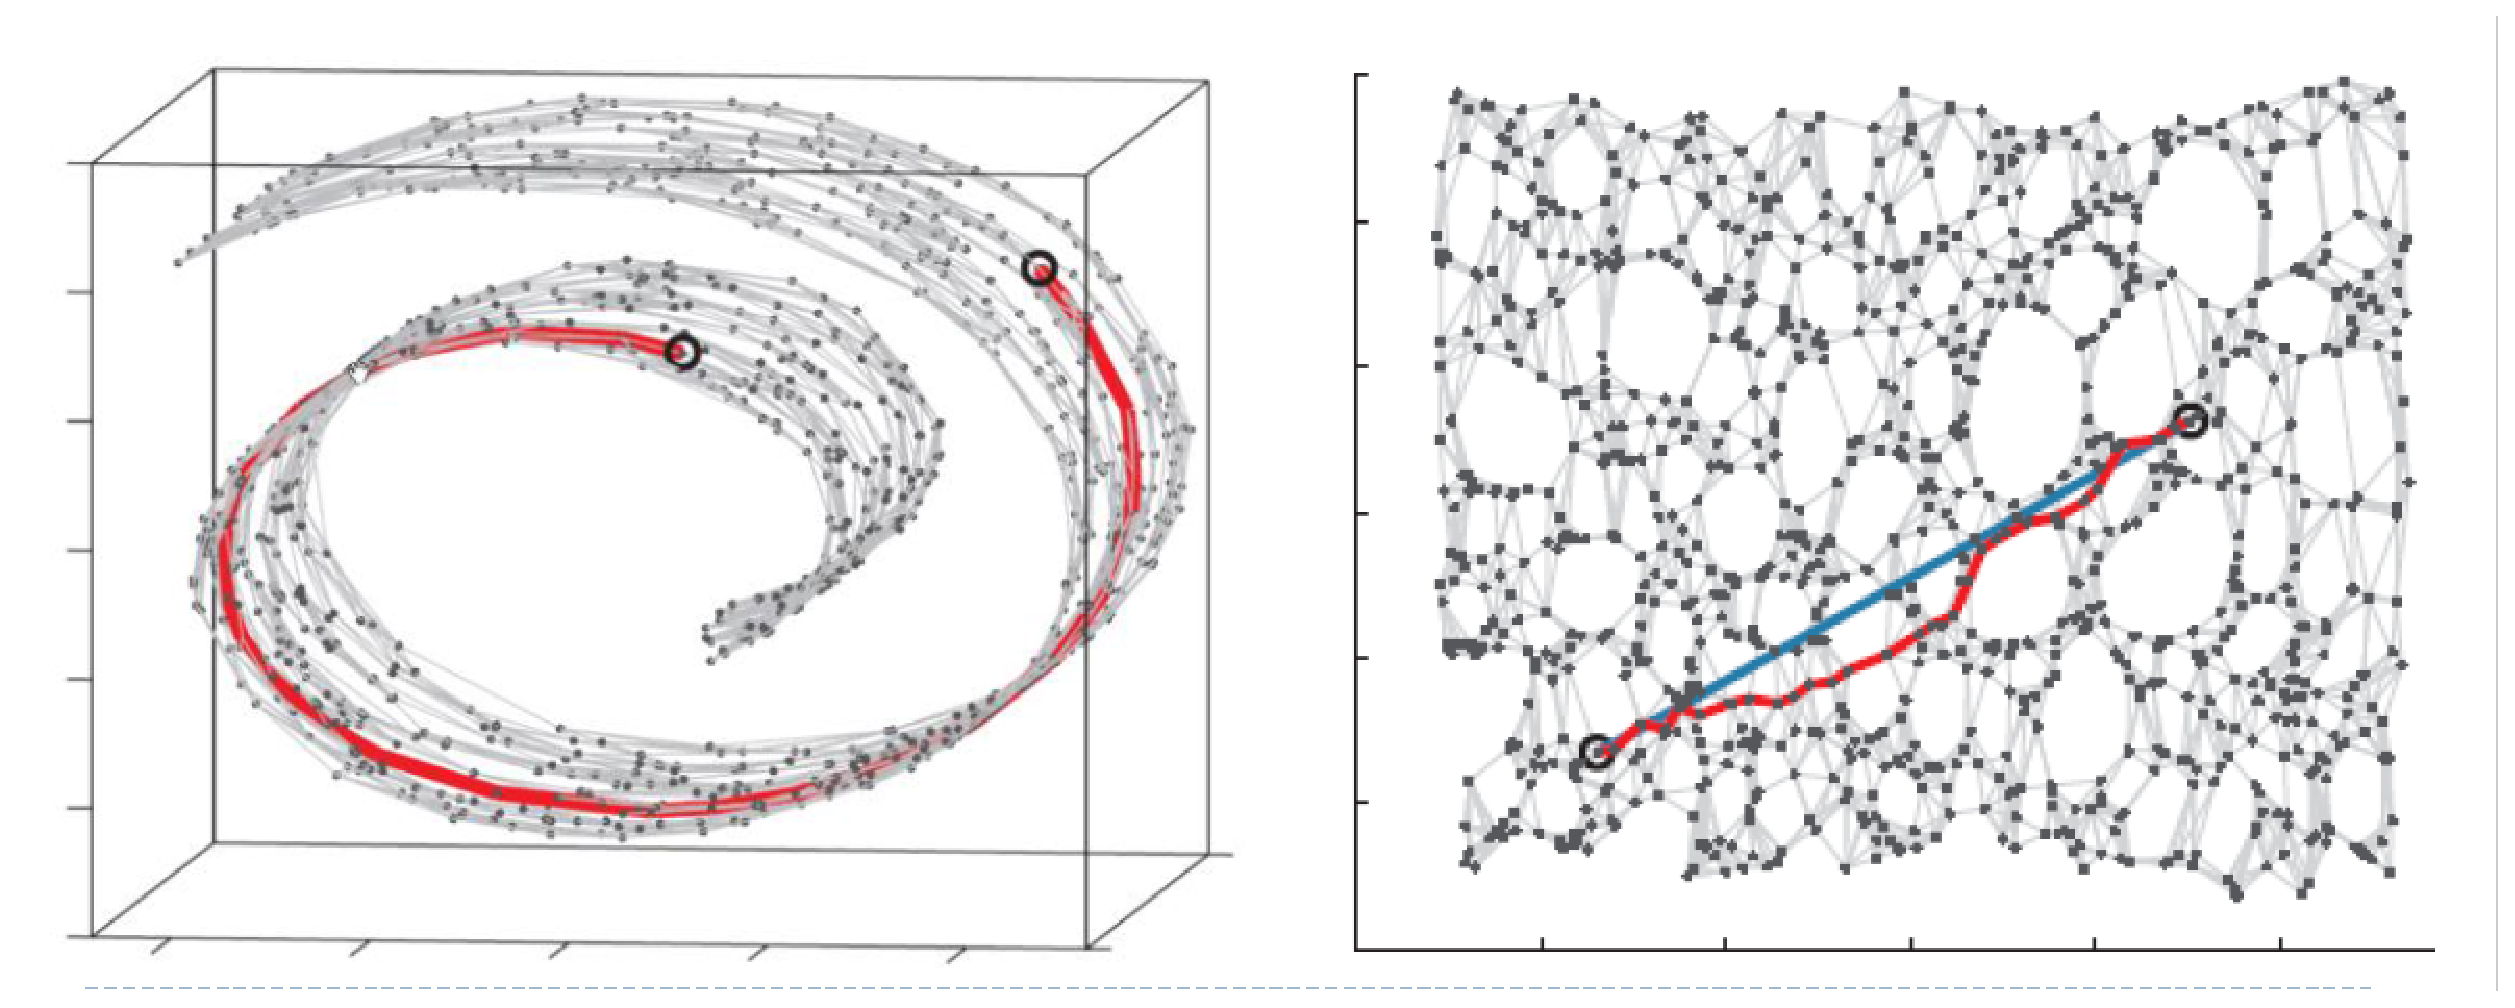
\includegraphics[scale=0.2]{./figs/fig6.eps}
   	\end{figure}
    \end{frame}
    
    \subsection{Local Linear Embedding}
    \begin{frame}{Local Linear Embedding}
    \alert{Local Linear Embedding}(2000 Science) is another famous manifold learning method. It tries to preserve the local linear relationship.
    \begin{figure}
    \centering
    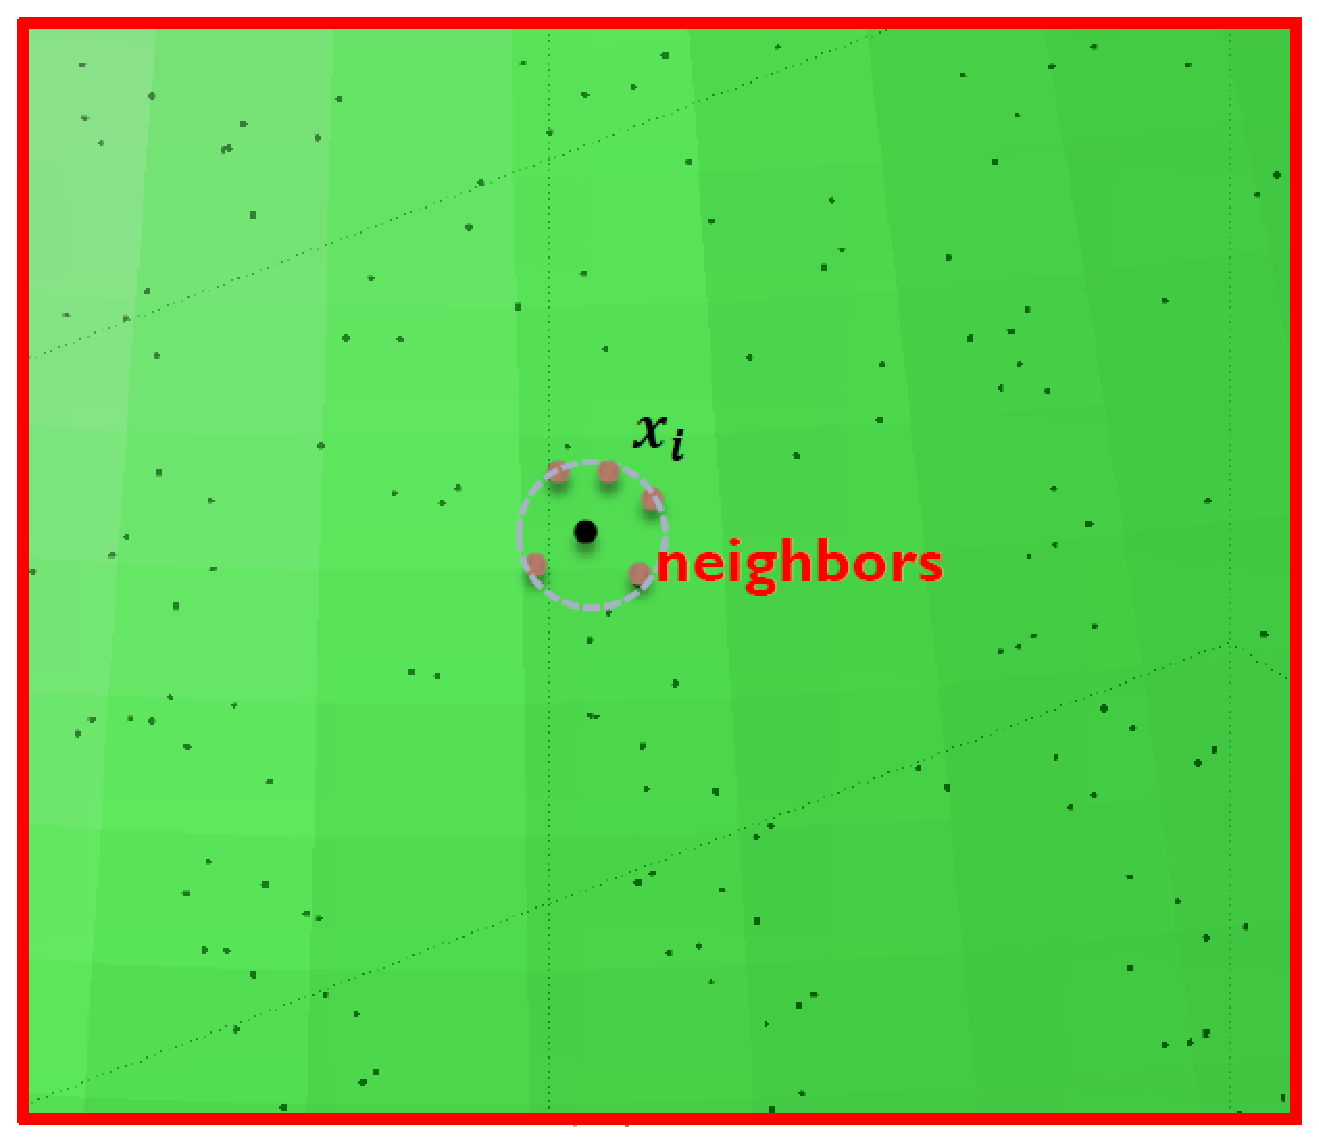
\includegraphics[scale=0.2]{./figs/fig7.eps}
    \end{figure}
    \vspace{-5mm}
     \begin{eqnarray*}
    	\min\epsilon(W) & = & \min\sum_i\Vert \bol{x}_i - \sum_jW_{ij}\bol{x}_j \Vert \\
    							 &     & s.t. \sum_j W_{ij} = 1
    \end{eqnarray*}
    \end{frame}
    
    \begin{frame}{Local Linear Embedding}
    \alert{Local Linear Embedding}(2000 Science) is another famous manifold learning method. It tries to preserve the local linear relationship.
    \begin{figure}
    \centering
    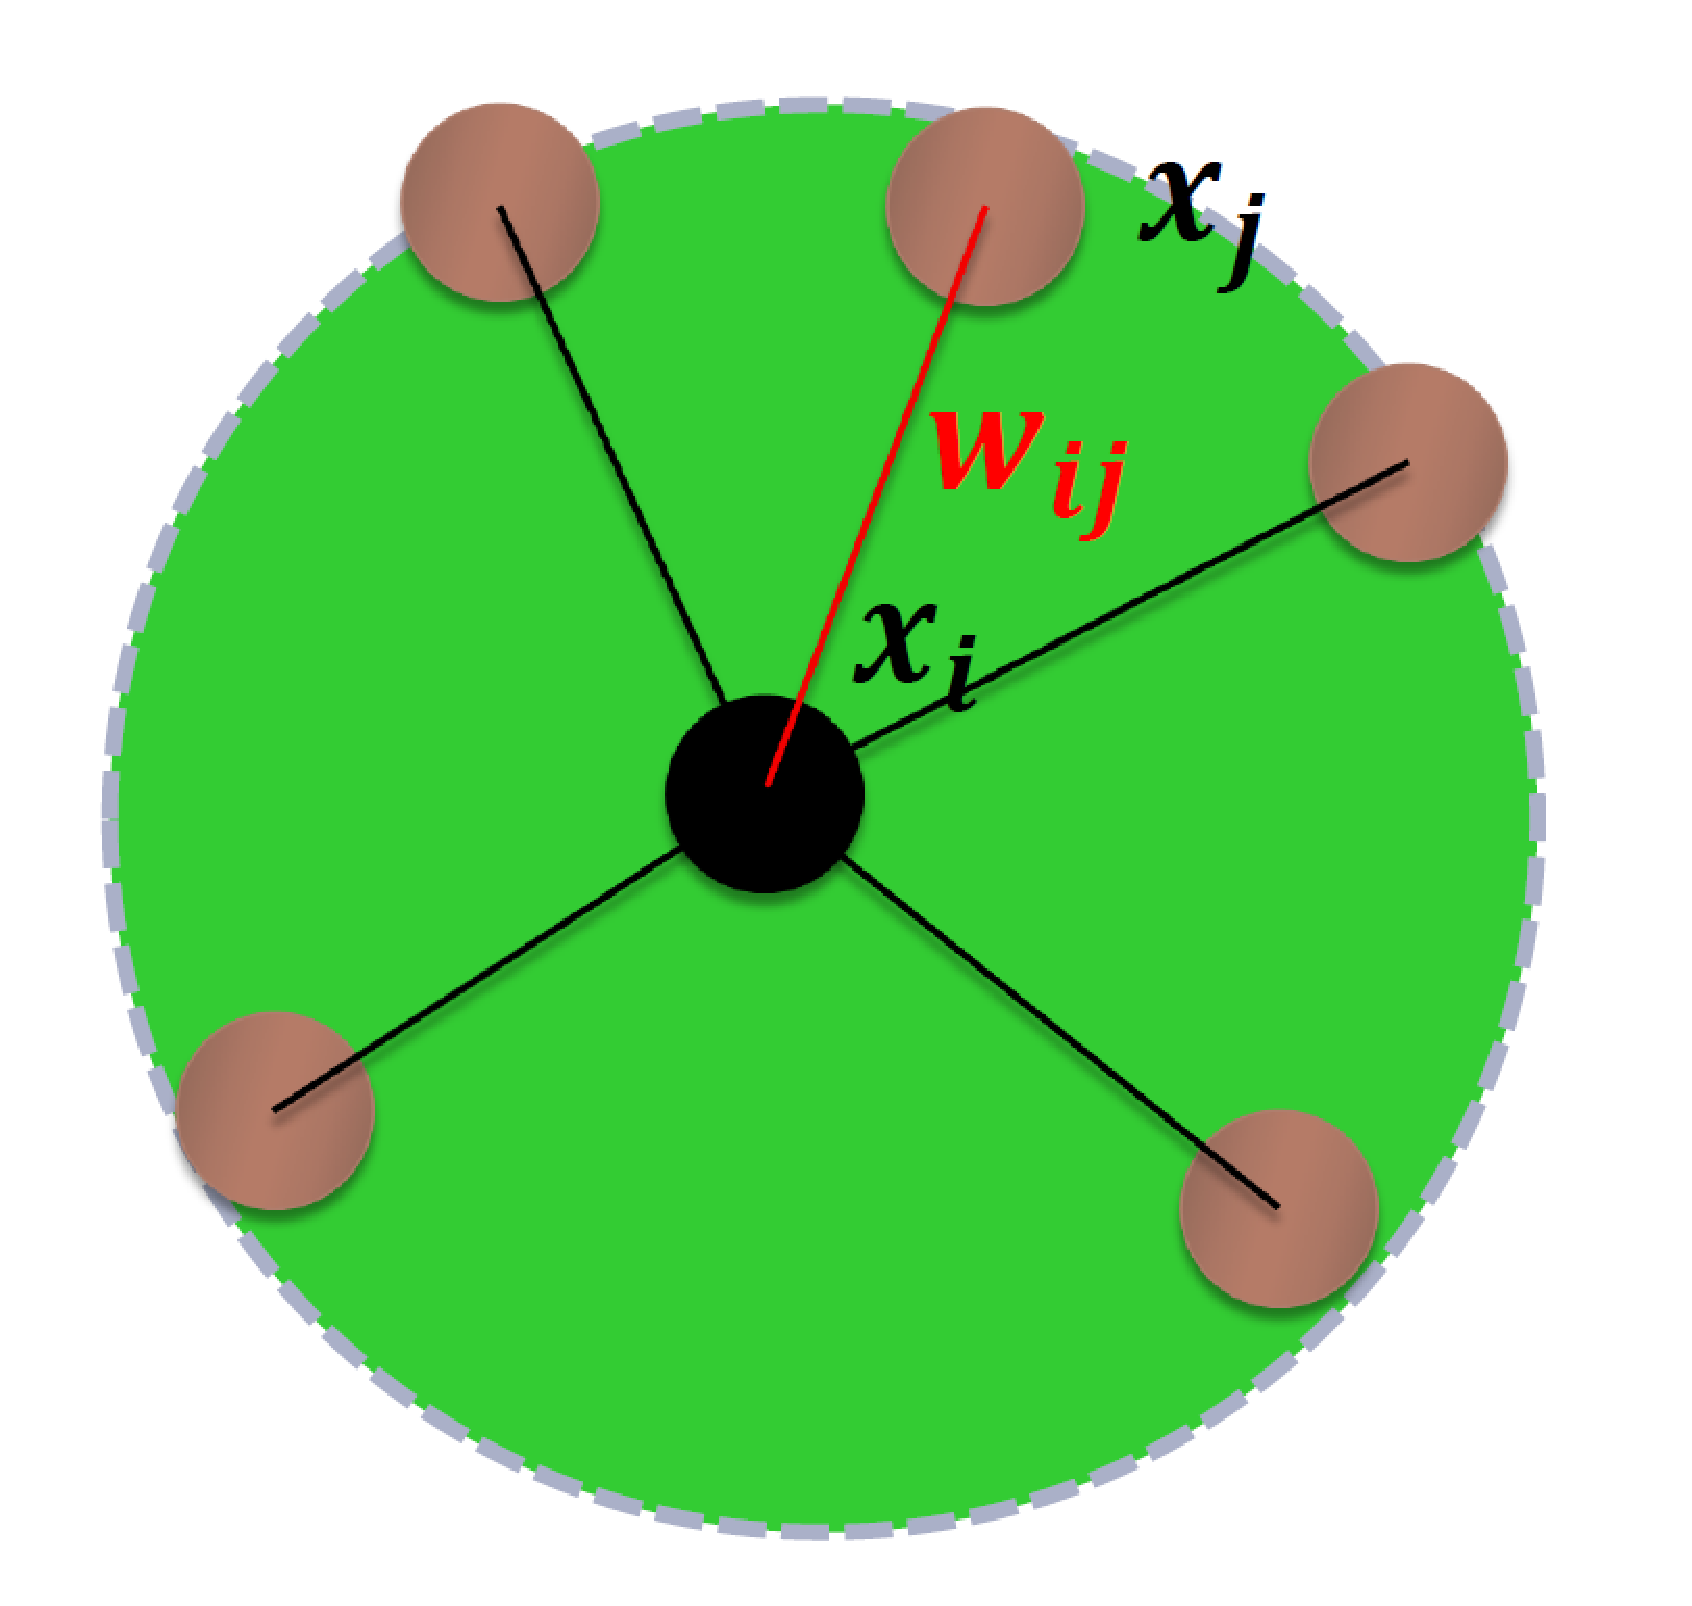
\includegraphics[scale=0.15]{./figs/fig8.eps}
    \end{figure}
	\begin{displaymath}
	\min\Phi(\bol{y}) = \min\sum_i\Vert \bol{y}_i - \sum_jW_{ij}\bol{y}_j  \Vert^2
	\end{displaymath}
    \end{frame}
    
    
    \subsection{Laplacian Eigenmaps}
    \begin{frame}{Laplacian Eigenmaps}
    In Laplacian Eigenmaps, a conclusion has been proofed: \\
    \begin{displaymath}
    	\vert f(\bol{z} ) - f(\bol{x})\vert < \Vert \nabla f(\bol{x}) \Vert\cdot \Vert \bol{z} - \bol{x} \Vert + o(\Vert \bol{z} - \bol{x} \Vert)
    \end{displaymath}
    \begin{itemize}
    \item If $\bol{x}_i$ and $\bol{x}_j$ are close to each other and the gradient of map $f$ is small, we can sure that $f(\bol{x}_i)$ and $f(\bol{x}_j)$ preserve local structure.
    \end{itemize}
    Construct Laplace matrix and get object function
    \begin{displaymath}
    	\min_{\Vert f \Vert_{L^2(\mathcal{M})} = 1}\int_{\mathcal{M}}\Vert\nabla f(\bol{x})\Vert^2 \Rightarrow\min\sum_{i,j}(y_i - y_j)^2W_{ij} \Rightarrow L\bol{y} = \lambda D\bol{y}
    \end{displaymath}
    \end{frame}
    
    \begin{frame}{Laplace Operator on Graph}
    \begin{itemize}
    	\item L is the Laplace operator, which measures the smooth of the function on manifold
    	\item On Graph, L is Laplace matrix
    \end{itemize}
    \begin{figure}
    \centering
    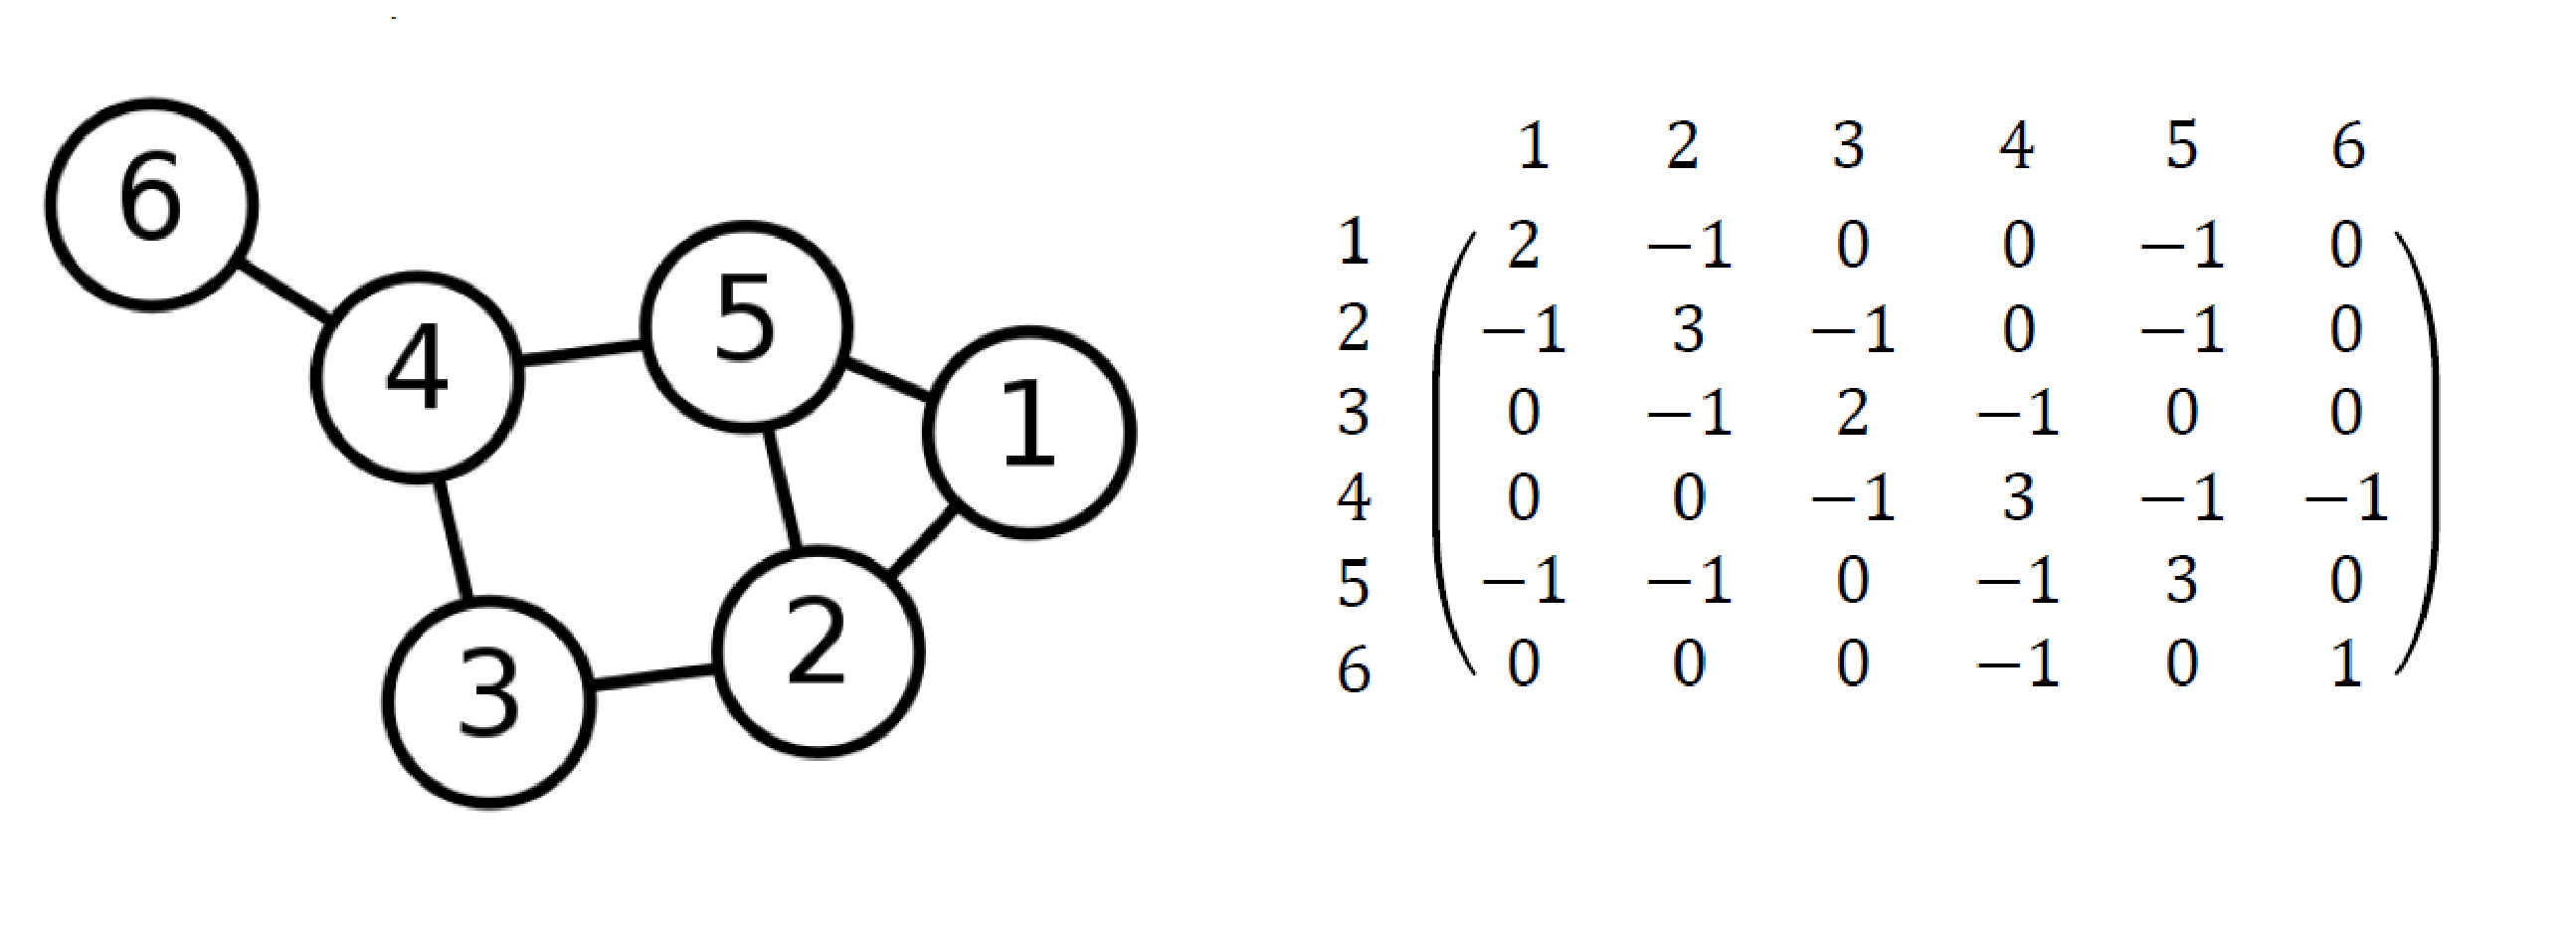
\includegraphics[scale=0.2]{./figs/fig9.eps}
    \end{figure}
    \end{frame}
    
    
    
	\begin{frame}{Global vs Local}
	\begin{itemize}
		\item Global method : ISOMAP\\
		\item Local method : LLE, LE\\
		\item Global method can keep more informations of data\\
		\item But large amount of computation
	\end{itemize}
	\end{frame}	    
    
    \begin{frame}{Out of sample problem}
    \begin{itemize}
    	\item LE and LLE can not applied on new samples. 
    	\item Use linear projection: $y = \bol{p}^T\bol{x}$
    	\item LE$\Rightarrow$ LPP : $XLX^T\bol{p} = \lambda XDX^T\bol{p}$
    	\item LLE$\Rightarrow$ NPE : $XMX^T\bol{p} = \lambda XX^T\bol{p}$
    	\item Projection Matrix $P = [\bol{p}_1, \ldots, \bol{p}_d]$
    	\item Given a new sample $\bol{y}$, we can project it to low-dim space $\bol{z} = P^T\bol{y}$
    \end{itemize}
    
    \end{frame}
    
   \subsection{Vector Field based Dimensionality Reduction}
   \begin{frame}{Vector Field based Dimensionality Reduction}
   \framesubtitle{Parallel Vector Field Embedding}
   The goal to find a map $F=(f_1,\ldots,f_d) : \mathcal{M} \subset \mathbb{R}^n \to \mathbb{R}^d$
   \begin{itemize}
   	\item $F$ is a local isometry
   	\item $dF$ is orthonormal
   	\item $df_i$ is parallel vector fields $\Rightarrow$ $\nabla df_i = 0$
   \end{itemize}
   Steps:
   \begin{enumerate}
   	\item $\displaystyle E(V) = \int_{\mathcal{M}}\Vert \nabla V \Vert^2dx,\quad  s.t. \int_{\mathcal{M}}\Vert V \Vert^2=1$
   	\item $\displaystyle\min\Phi(f) = \int_{\mathcal{M}}\Vert \nabla f - V \Vert^2dx$
   \end{enumerate}
   \alert{A new perspective for manifold learning}
	\end{frame}      
   
   \begin{frame}{Swiss Roll}
   \begin{figure}
   \centering
   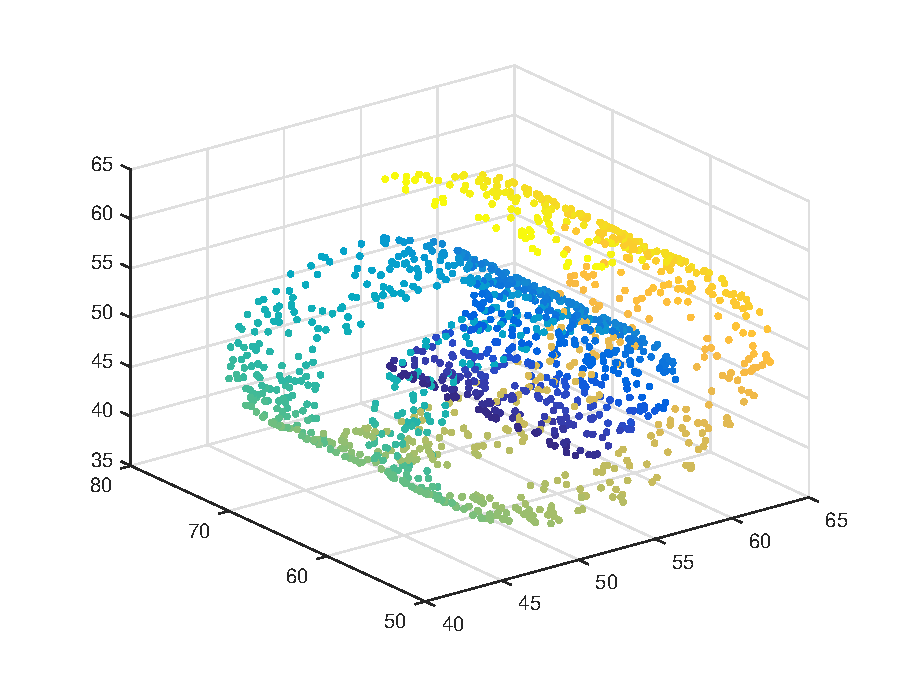
\includegraphics[scale=0.5]{./figs/swiss.eps}
   \caption{Swiss Roll}
   \end{figure}
   \end{frame}
   
   
   \begin{frame}{PFE}
   \begin{figure}
   \centering
   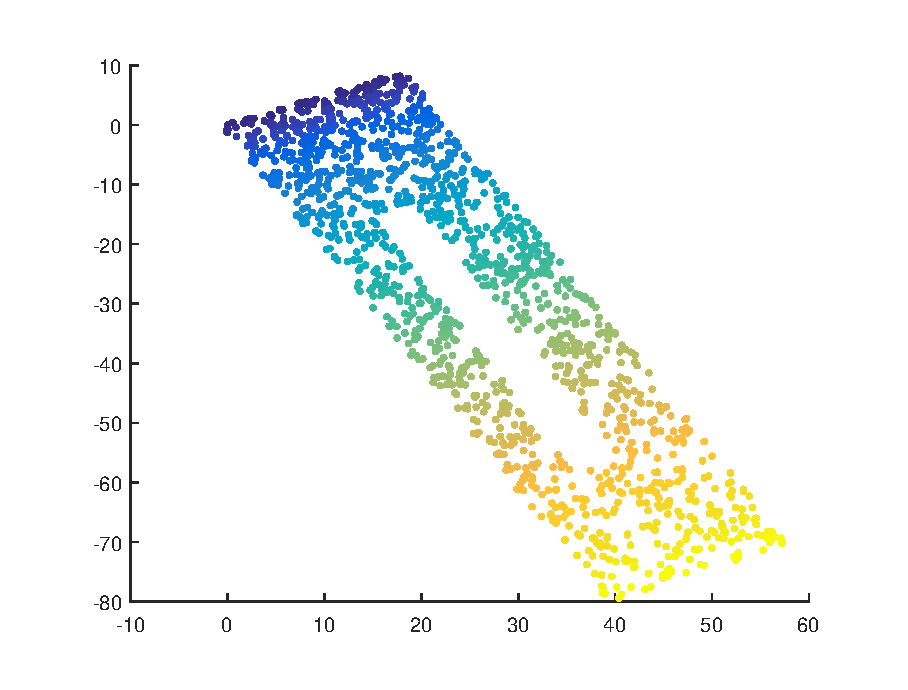
\includegraphics[scale=0.5]{./figs/pfe.eps}
   \caption{PFE}
   \end{figure}
   \end{frame}
   
   
   \begin{frame}{PCA}
   \begin{figure}
   \centering
   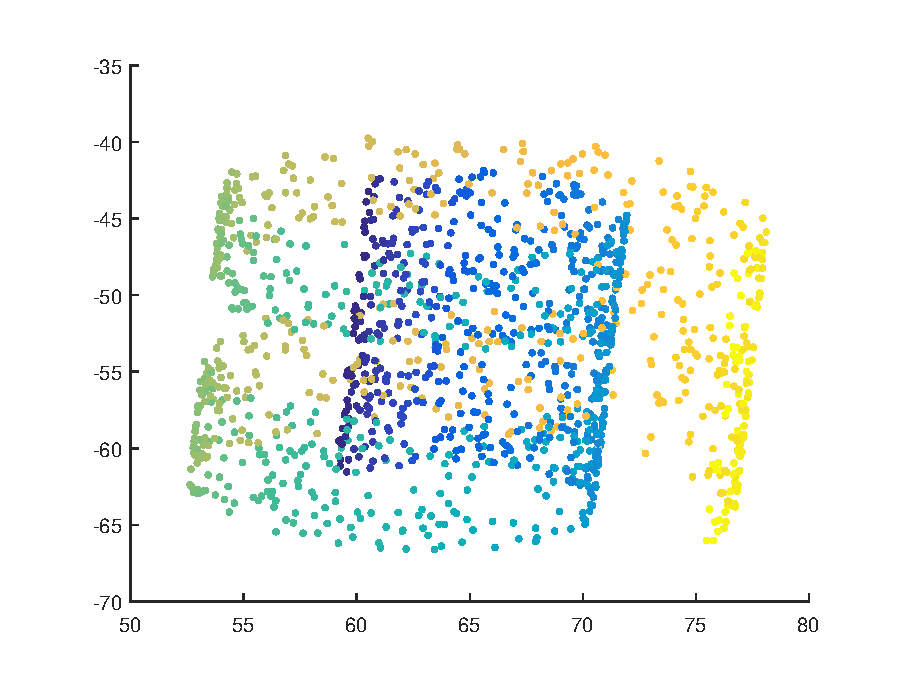
\includegraphics[scale=0.5]{./figs/pca.eps}
   \caption{PCA}
   \end{figure}
   \end{frame}
   
   \begin{frame}{ISOMAP}
   \begin{figure}
   \centering
   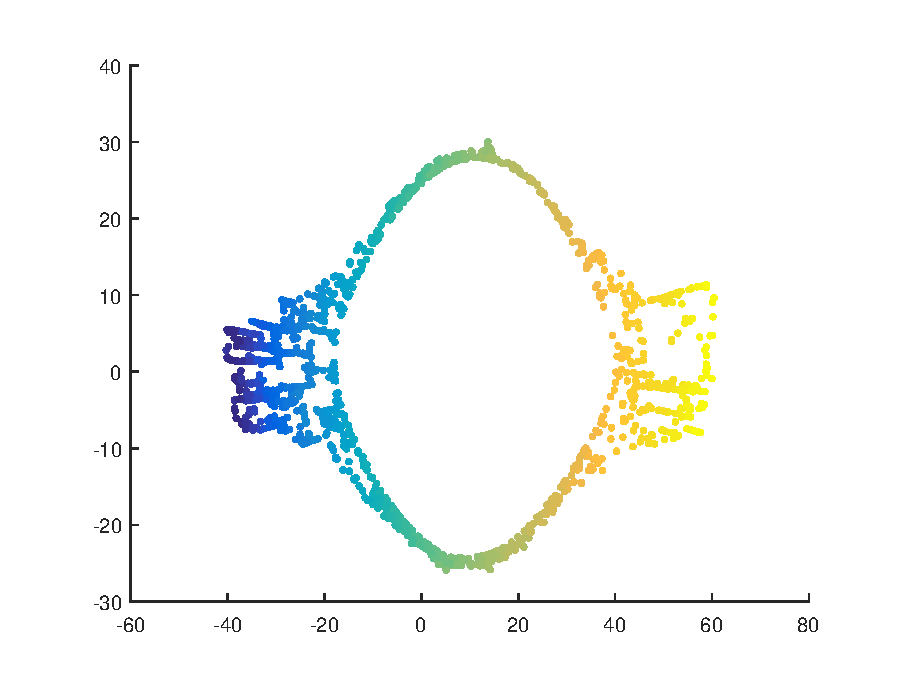
\includegraphics[scale=0.5]{./figs/isomap.eps}
   \caption{ISOMAP}
   \end{figure}
   \end{frame}   
   
   \begin{frame}{LLE}
   \begin{figure}
   \centering
   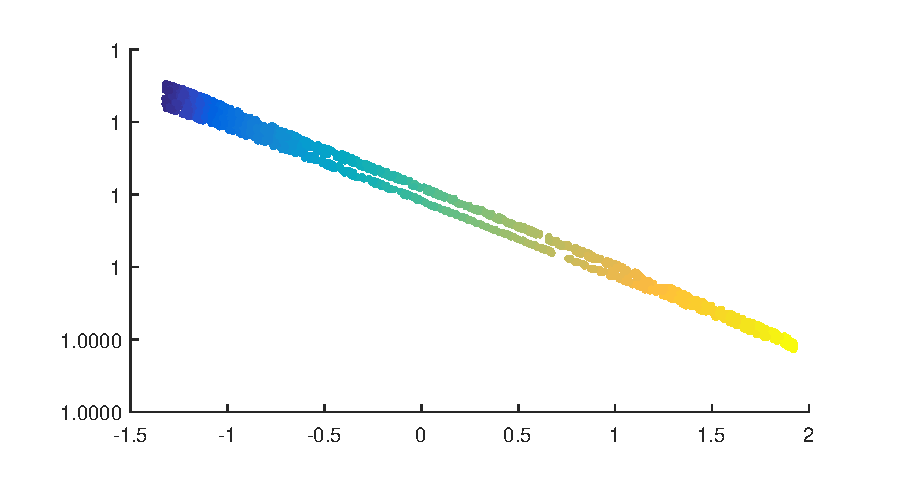
\includegraphics[scale=0.5]{./figs/lle0.eps}
   \caption{LLE}
   \end{figure}
   \end{frame}
   
   
   \begin{frame}{LE}
   \begin{figure}
   \centering
   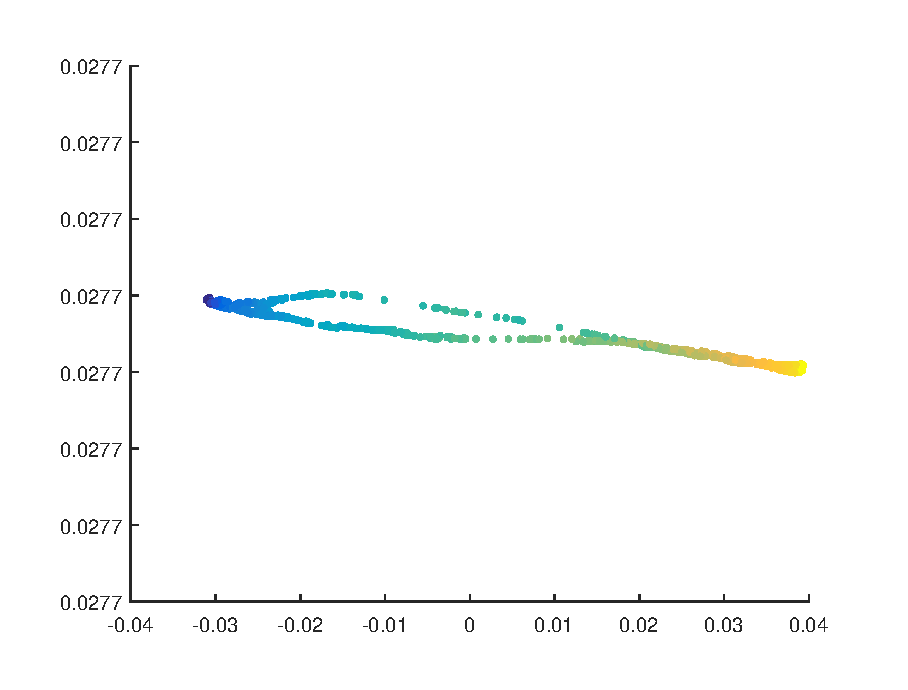
\includegraphics[scale=0.5]{./figs/le5.eps}
   \caption{LE}
   \end{figure}
   \end{frame}
   
   \begin{frame}{NPE}
   \begin{figure}
   \centering
   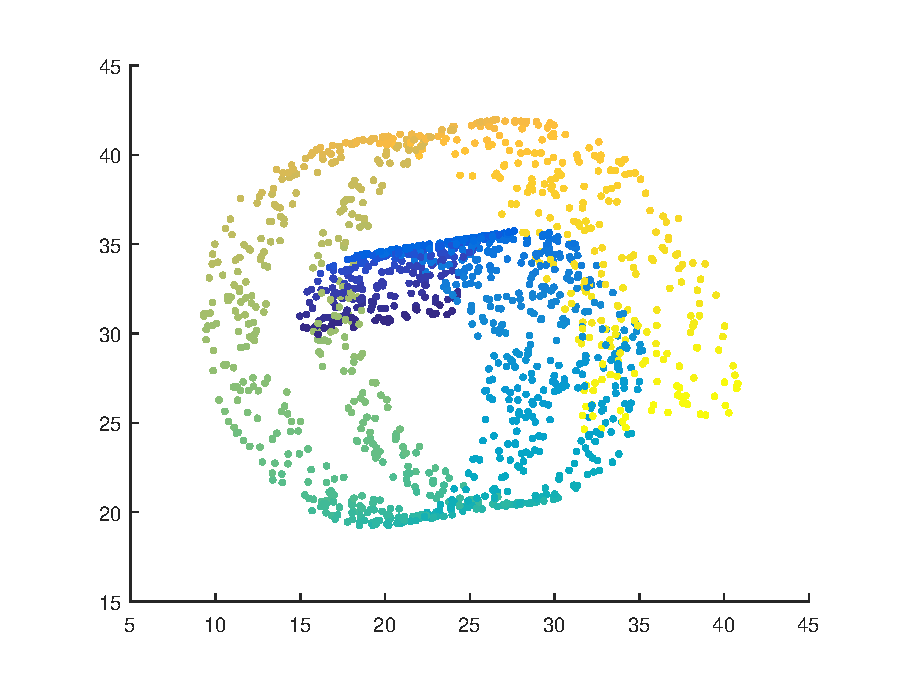
\includegraphics[scale=0.5]{./figs/lle.eps}
   \caption{NPE}
   \end{figure}
   \end{frame}
   
   \begin{frame}{LPP}
   \begin{figure}
   \centering
   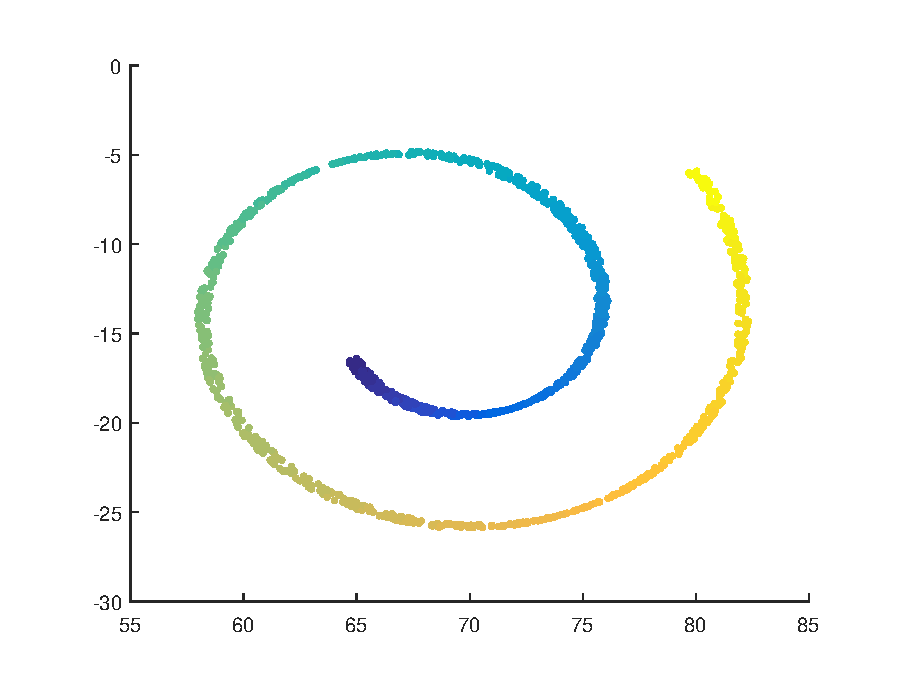
\includegraphics[scale=0.5]{./figs/lpp.eps}
   \caption{LPP}
   \end{figure}
   \end{frame}
   
   \section{Manifold Regularization : Semi-Supervised Setting}
   \begin{frame}{Manifold Regularization}
   \begin{itemize}
   	\item \alert{Measured (labeled)} points: discriminant structure\\
   	\begin{displaymath}
   		\min\sum_{i = 1}^k\left(y_i - f(\bol{z}_i)\right)^2
   	\end{displaymath}
	\item \alert{Unmeasured (unlabeled)} points: geometrical structure\\
	\begin{displaymath}
		\min\sum_{i,j}\left(f(\bol{x}_i) - f(\bol{x}_j)\right)^2S_{ij}
	\end{displaymath}
   \end{itemize}
   \begin{displaymath}
   		\min_f\sum_{i = 1}^k\left(y_i - f(\bol{z}_i)\right)^2 + \frac{\lambda}{2}\sum_{i,j}^m\left(f(\bol{x}_i) - f(\bol{x}_j)\right)^2S_{ij}
   \end{displaymath}
   \end{frame}
   
  \begin{frame}{Laplacian Regularized Least Square}
  \begin{itemize}
  \item Linear objective function
  \begin{displaymath}
  	\min_{\bol{w}}\sum_{i=1}^k\left( y_i - \bol{w}^T\bol{z}_i \right) + \frac{\lambda_1}{2}\sum_{i,j=1}^m\left(  \bol{w}^T\bol{x}_i - \bol{w}^T\bol{x}_j  \right)^2S_{ij} + \lambda_2\Vert\bol{w}\Vert
  \end{displaymath}
  \item Solution
  \begin{displaymath}
  	\widehat{\bol{w}} = \left(  ZZ^T + \lambda_1XLX^T + \lambda_2I  \right)^{-1}Z\bol{y}
  \end{displaymath}
  \item $Z=(\bol{z}_1,\ldots,\bol{z}_k)$ : labeled points
  \item $X=(\bol{x}_1, \ldots, \bol{x}_m)$: all points
  \end{itemize}
  \end{frame}
  
  \begin{frame}{Parallel Field Regularization}
  \begin{displaymath}
  	\arg\min_{f,V} E(f, V) = \frac{1}{m}\sum_{i=1}^m R_0(\bol{x}_i, y_i, f) + \lambda_1 R_1(f,V) + \lambda_2 R_2(V)
  \end{displaymath}
  Where
  \begin{itemize}
  	\item $\displaystyle R_1(f,V) = \int_{M}\Vert \nabla f - V \Vert^2$, \qquad $\displaystyle R_2(V) = \int_{M}\Vert \nabla V \Vert^2$
  	\item Low cost of estimation.
  	\item Insensitive to noise.
  \end{itemize}
  \end{frame}
  
  
  
  \begin{frame}{Resources}
  Conference:
  \begin{itemize}
  	\item Computer Vision: CVPR, ICCV, ECCV
  	\item Machine Learning: NIPS, ICML, IJCAI, AAAI
  	\item NLP : ACL
  \end{itemize}
  
  Journal:
	\begin{itemize}
		\item IEEE Trans on Pattern Analysis and Machine Intelligence(TPAMI)
		\item Journal of Machine Learning Research(JMLR)
		\item International Journal of Computer Vision(IJCV)
	\end{itemize}	  
  
  Tools:
  \begin{itemize}
  	\item Scikit-learn: http://scikit-learn.org/
  	\item OpenCV: https://opencv.org/
  \end{itemize}
  \end{frame}
    \begin{frame}
		\centering\Huge{Thanks !}\\
		\centering\Huge{Q\&A}
	\end{frame}	  
    \end{darkframes}
\end{document}
